\newpage
\section{Dreidimensionales Punktediagramm}

Falls Datensätze mit einer unabhängigen und zwei abhängigen Variablen dargestellt werden sollen, kann ein dreidimensionales Punktediagramm verwendet werden.

Beispiele für Datensätze, die in dreidimensionalen Punktediagrammen dargestellt werden können:

\begin{itemize}
	\item Zwei Attribute im Laufe der Zeit, zum Beispiel BIP und Anstellung eines Landes
	\item Drei Attribute, die in einem bestimmten Verhältnis zueinander stehen. Zum Beispiel Geschwindigkeit, Luftwiderstand, Oberfläche
\end{itemize}

Es wurde entschieden, eine weitere Applikation zu entwickeln, die einen Datensatz mit einer unabhängigen und zwei abhängigen Variablen in einer 3D-Applikation anzeigt.

\subsection{Applikation}

\begin{figure}[!htbp]
	\centering
	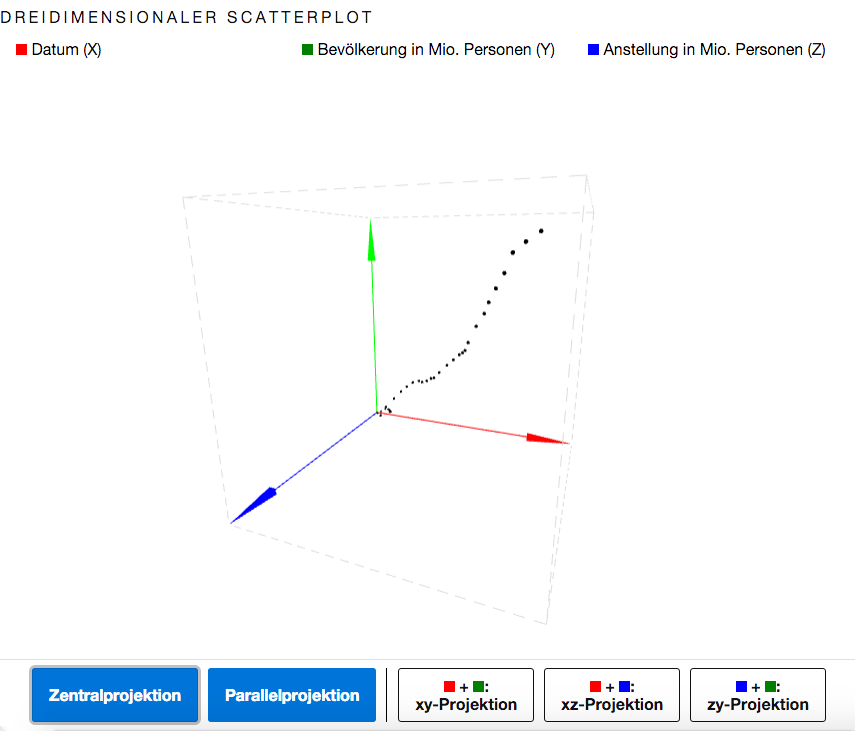
\includegraphics[width=\linewidth]{images/3d}
	\caption{Oberfläche der Applikation (dreidimensionales Punktediagramm)}
	\label{fig:3d}
\end{figure}

Die Applikation wurde mit der Programmierbibliothek \textit{Three.js} erstellt. Three.js ermöglicht die Entwicklung von 3D-Applikationen mit JavaScript im Browser.

\textbf{Achsen.} Als Achsen wurden verschiedenfarbige Pfeile (Abbildung \ref{fig:vectors}) mit Richtungsvektoren $\vec{a}_x$, $\vec{a}_y$, $\vec{a}_z$ erstellt.

\begin{figure}[!htbp]
	\centering
	\begin{math}
		\vec{a}_x=\begin{pmatrix} 1 \\ 0 \\ 0 \end{pmatrix} \qquad
		\vec{a}_y=\begin{pmatrix} 0 \\ 1 \\ 0 \end{pmatrix} \qquad
		\vec{a}_z=\begin{pmatrix} 0 \\ 0 \\ 1 \end{pmatrix} \qquad
	\end{math}
	\caption{Die Richtungsvektoren der Achsen im dreidimensionalen Punktediagramm.}
	\label{fig:vectors}
\end{figure}